%\documentclass[letterpaper]{report}
\documentclass[letterpaper]{article}
\title{\LaTeX\ \ tutorial}
\author{Cem Karan\\Aylin \c{C}al{\i}\c{s}kan}

%%%%%%%%%%%%%%%%%%%%%%%%%%%%%%%%%%%%%%%%%%%%%%%%%%%%%%%%%%%%%%%%%%%%%%%%%%%%%%%% 
% Latex is quite powerful, but it isn't all powerful.  There are a number of additional 
% packages that increase its power.  In order to import a package, you need to use 
% the '\usepackage' command. The \usepackage command is similar to #include in 
% C++ or import in other languages.  A good place to start looking for 
% packages is at: 
%
%		http://www.tug.org/ctan.html 
%
% Many of those packages are already installed on Eniac, so all you have to do is 
% call \usepackage to make use of them.
% 
% There is one difference between #include and \usepackage though; 
% \usepackage is more like a function invocation.  Several of the packages 
% below have a long series of arguments within the square brackets; look 
% up what those arguments are doing in the package documentation 
% referenced just above the \usepackage line. 
%%%%%%%%%%%%%%%%%%%%%%%%%%%%%%%%%%%%%%%%%%%%%%%%%%%%%%%%%%%%%%%%%%%%%%%%%%%%%%%%

% http://tug.ctan.org/cgi-bin/ctanPackageInformation.py?id=algorithm2e
\usepackage[algo2e, algoruled, vlined, linesnumbered, commentsnumbered, inoutnumbered, longend]{algorithm2e}

% http://tug.ctan.org/cgi-bin/ctanPackageInformation.py?id=hyperref
\usepackage[colorlinks]{hyperref}

% http://tug.ctan.org/cgi-bin/ctanPackageInformation.py?id=geometry
\usepackage[margin = 1in, paper = letterpaper]{geometry}

% http://tug.ctan.org/cgi-bin/ctanPackageInformation.py?id=amsfonts
\usepackage{amsfonts}

% http://tug.ctan.org/cgi-bin/ctanPackageInformation.py?id=amsmath
\usepackage{amsmath}

% http://tug.ctan.org/tex-archive/fonts/amsfonts/doc/
\usepackage{amssymb}

% http://tug.ctan.org/cgi-bin/ctanPackageInformation.py?id=bbm
\usepackage{bbm}

% http://tug.ctan.org/cgi-bin/ctanPackageInformation.py?id=color
\usepackage{color}

% http://tug.ctan.org/cgi-bin/ctanPackageInformation.py?id=enumerate
\usepackage{enumerate}

% http://tug.ctan.org/cgi-bin/ctanPackageInformation.py?id=graphicx
\usepackage{graphicx}

% http://www.tug.org/texmf-dist/doc/latex/base/latexsym.pdf
\usepackage{latexsym}

% http://www.tug.org/texmf-dist/doc/latex/base/makeindx.pdf
% http://www.mackichan.com/techtalk/505.htm
\usepackage{makeidx}

% http://tug.ctan.org/cgi-bin/ctanPackageInformation.py?id=multicol
\usepackage{multicol}

% http://tug.ctan.org/cgi-bin/ctanPackageInformation.py?id=subfig
\usepackage{subfig}

% http://tug.ctan.org/cgi-bin/ctanPackageInformation.py?id=xspace
\usepackage{xspace}

%%%%%%%%%%%%%%%%%%%%%%%%%%%%%%%%%%%%%%%%%%%%%%%%%%%%%%%%%%%%%%%%%%%%%%%%%%%%%%%% 
% Some systems understand PDF, while others understand EPS.  For example, 
% under OS X, if you use TeXShop, then you'll want your images to be PDF 
% images (This may work on Eniac, which used to only understand EPS files,
% but now appears to understand PDF as well (after 23 July 2010))
%
% In order to make it easy to switch between the two types, you can declare 
% what the file suffix is for all graphics that you want to include using 
% the \includegraphics{} command by setting 
% \DeclareGraphicsExtensions{.pdf}. So, if I've declared the extension to 
% be `.pdf', and I use the command `\includegraphics{RandomPicture}', 
% Latex will search for the file named `RandomPicture.pdf'.  Changing the 
% command to \DeclareGraphicsExtensions{.eps} means that Latex will search 
% for `RandomPicture.eps' instead. 
%%%%%%%%%%%%%%%%%%%%%%%%%%%%%%%%%%%%%%%%%%%%%%%%%%%%%%%%%%%%%%%%%%%%%%%%%%%%%%%% 
\DeclareGraphicsExtensions{.pdf} 
%\DeclareGraphicsExtensions{.eps}

%%%%%%%%%%%%%%%%%%%%%%%%%%%%%%%%%%%%%%%%%%%%%%%%%%%%%%%%%%%%%%%%%%%%%%%%%%%%%%%%
% Document start
% 
% Everything above the `\begin{document}' command is in an area called 
% the preamble.  Much like HTML, the preamble occurs in the header section, 
% while the body occurs within the `\begin{document}' section.  Note that if 
% you scroll to the very end, you will find a `\end{document}' command.  
% LaTeX requires all `\begin{...}' commands to be closed with `\end{...}' 
% commands, and it requires that they nest properly.  If you forget a closing 
% \end, your document will have errors.
%%%%%%%%%%%%%%%%%%%%%%%%%%%%%%%%%%%%%%%%%%%%%%%%%%%%%%%%%%%%%%%%%%%%%%%%%%%%%%%%

\begin{document}

\maketitle
\tableofcontents

\section*{Preface}

This is an extremely brief tutorial on \LaTeX, intended to get you up 
and running quickly on Eniac.  If you are currently reading the PDF 
version of this file, \emph{be sure} to download the \LaTeX\ version of 
this file and read it as well.  The best way to learn a new language is 
to read through examples of it, and then to experiment with it, and this 
tutorial is written with the intention and expectation that you 
\emph{will} download and read the \LaTeX\ version of the file in 
addition to the PDF version.  Quite a bit of what you read in the PDF 
file will be unintelligible without the \LaTeX\ file! The \LaTeX\ 
version is called \verb+LaTeX_Tutorial.tex+.  As an aside, the file 
suffix for \LaTeX\ is usually\verb+.tex+.

\pagebreak
\section{Resources}

The following are excellent resources on \LaTeX.

\begin{itemize}

\item 
\href{http://www.amazon.com/LaTeX-Document-Preparation-System-2nd/dp/0201529831}
{\underline{LaTeX: A Document Preparation System (2nd Edition)}} This 
is one of two books that everyone always refers to when they want to 
learn or do anything with \LaTeX.  Note that it is the short one; the other, 
\href{http://www.amazon.com/LaTeX-Companion-Techniques-Computer-Typesetting/dp/0201362996}
{\underline{The LaTeX Companion (Tools and Techniques for Computer Typesetting)}} 
is much more comprehensive, but also more than you will likely ever 
want or need.

\item \href{http://www.latex-project.org/}{LaTeX--A document preparation system} 

Not to be confused with the book of the same name, 
this is the main site for \LaTeX.  Ignore the LaTeX3 information; the 
only version available anywhere is \LaTeX\ 2$\epsilon$.  Note that the 
language itself has not changed, so that information is still valid.

\item \href{http://www.tug.org/}{\TeX\ User's Group} - \TeX\ is the 
language that underlies \LaTeX.  This site is dedicate to both \LaTeX\ 
and \TeX, and has extensive documentation on various packages that you 
can use, as well as tutorials that you can look through.

\item \href{http://www.tug.org/ctan.html}{CTAN} - The Comprehensive 
\TeX\ Archive Network.  This is where you will go if you are looking for 
more packages to use.  Packages are exactly what they sound like; things 
that you include via the \verb+\usepackage{}+ command.  See the start of 
the \verb+LaTeX_Tutorial.tex+ file for a whole list of packages that 
this file has included.  Note that if you include it but don't use it, 
you're not costing yourself anything.  The easiest way to handle 
packages is to leave all the ones that you use regularly in some \LaTeX\ 
file, and copy them over.  For example, grab the 
\verb+LaTeX_Tutorial.tex+ itself, get rid of the parts you don't need, 
and use the rest.  That's what it's there for! :)

\end{itemize}

\section{Running \LaTeX}

This tutorial assumes that you are going to run under Eniac, via the 
command line.  There are packages available for Windows and OS X, but 
you will need to install and learn how to use them yourself; there 
isn't enough space in this tutorial to explain how to install and use packages
on other systems.

Take the \LaTeX\ version of this file and put it somewhere convenient 
that you have write access to that is reachable from the Eniac.  Note 
that \LaTeX\ generates a lot of intermediate files, so if you want to be 
able to quickly get rid of everything, it is probably best to create an 
new, empty directory somewhere, and run everything from there.

Log into Eniac, change directories to somewhere convenient, and extract 
the tarball that contains this \LaTeX\ file and all of its associated 
files.  Note that the tarball has had all of the temporary files 
removed; if you plan on using version control, now is a good time to 
note what files you have, and to compare it to the files you will have 
after \LaTeX\ is done running.  Whatever gets generated by \LaTeX\ can 
be safely disposed of because \LaTeX\ will regenerate it later on.  For 
the time being, I'm going to assume that you have a directory named 
\texttt{LaTeX\_Tutorial} that you are operating out of.  If you just 
untar the tarball, it should create that directory for you.

\begin{enumerate}

\item Change directories to the \texttt{LaTeX\_Tutorial} directory.

\item Run \texttt{latex LaTeX\_Tutorial.tex} from the command line.  
This will generate many files, including a \texttt{.dvi} file.  
\texttt{.dvi} files are device independent files.  They are like the 
great-granddaddy of PDF, PS, EPS, etc.  Once a \LaTeX\ file has been 
compiled into a \texttt{.dvi} file, other tools can convert it into any 
number of other formats, including what we're going to do, which is PDF.

\item Run \texttt{dvipdf LaTeX\_Tutorial.dvi}.  This will generate the 
file \texttt{LaTeX\_Tutorial.pdf}.  If you're curious as to what 
other output forms you can render to, take a look in \texttt{/user/bin} 
for programs starting with \texttt{dvi}.  There are also a couple of 
\LaTeX\ programs that you might want to look at as well. They start with 
the name \texttt{latex}.

\end{enumerate}

A note about references, table of contents, indices, etc.  In 
section~\ref{Cross References} I'll tell you about the \verb+\label{}+ 
and \verb+\ref{}+ commands.  These create links within a document, 
including automatically generated section numbering.  The problem is how 
these references are generated; it requires two passes of \LaTeX\ to get 
them right.  If you see that everywhere you've used the \verb+\ref{}+ 
command you have \texttt{??} instead of actual numbers \& sections, or 
if you're missing your table of contents \& index, just run \LaTeX\ 
again.  It should fix all the references then.  Also, if you type in 
enough text that some items move to a different page, or if you reorder 
your sections, you will need to run the \verb+latex+ command twice.

A final note about running \LaTeX.  Given enough time and hacking, your 
\LaTeX\ file can get large, and you can end up with a lot of auxiliary 
files, especially if you use anything like 
\href{http://www.graphviz.org/}{GraphViz} or other tools to 
automatically generate images.  Create a \texttt{Makefile}, and use 
\texttt{make}. This will keep the headaches to a minimum, and it makes 
it easy to clean your files when you just want to get rid of all the 
dribbled bits that \LaTeX\ leaves behind.  It will also allow you to run 
the \verb+latex+ command twice as mentioned above.

\section{Basics}

\LaTeX\ uses a model similar to HTML + CSS; you mark up your document, 
delimiting blocks of text with special markup, which are then 
interpreted by \LaTeX\ along with some style files to determine how to 
render your document.  There are a number of built-in styles, and you 
can create your own.  Since this is supposed to be a brief tutorial, we 
won't go into how to write your own style files.  The important 
take-home point is that what you type in your document doesn't look 
anything like what will be finally outputted. Get used to writing some, 
and rendering some.

You can break up your document into chapters, sections, subsections, 
subsubsections.  Note that you will only have access to the chapter 
command if your document is a report.  If it is an article, you'll have 
access to everything except the chapter command.  As you might guess, 
chapters contain sections, which contain subsections, etc.  The commands 
always fall into two types; one which generates a chapter or section 
number, and one which doesn't.  The difference is the * character; 
unnumbered sections have it, numbered ones don't. In addition, each of 
the commands accepts an argument that is the name you want to give the 
sections.  As an example, I'm going to create several of these, which 
will generate a whole bunch of dummy sections. Read 
\texttt{LaTeX\_Tutorial.tex} to see how these work; reading the PDF file
will make no sense what-so-ever for these examples (everything in
\S\ref{Label for a numbered section start}).

% If you go to the top of this file, and change the comments so that 
% this is a report instead of an article, then the \chapter command will 
% work 
%\chapter{Dummy}

\section{This is the start of a numbered section}
\label{Label for a numbered section start}

\subsection{This is the start of a numbered subsection}
\label{Label for a numbered subsection start}

\subsubsection{This is the start of a numbered subsubsection}
\label{Label for a numbered subsubsection start}

\section*{This is the start of an unnumbered section}
\label{Label for an unnumbered section start}

\subsection*{This is the start of an unnumbered subsection}
\label{Label for an unnumbered subsection start}

\subsubsection*{This is the start of an unnumbered subsubsection}
\label{Label for an unnumbered subsubsection start}

Sections do not have an \verb+\end{}+ command; instead, a section will
continue until the next sectioning command.

Paragraphs are delimited by leaving a blank line between two blocks of 
text.  If you don't understand what I mean, \emph{start reading the} 
\texttt{LaTeX\_Tutorial.tex} \emph{file \textbf{now}}.

Notice that unnumbered sections (ones that have a `*' character) will 
not show up in the table of contents.  If you look at the unnumbered 
sections above, and look for them in the table of contents, you'll see 
what I mean.

\section{Environments}

Unlike many programming languages, \LaTeX\ is not context-free.  You can 
tell it to switch modes of behavior, which change what different 
characters and commands mean at a moment's notice. These modes are 
called \textbf{environments}.  Some environments are built-in, while 
others are supplied by packages that you include via the 
\verb+\usepackage+ command.  When you change to a new environment, 
you're getting a whole new set of rules, options, etc., that you can play 
with.  As a simple example, you can write extremely complicated 
mathematical equations using \LaTeX, but to do so, you must be in the 
math environment.  Environments that come in from other packages are 
usually well behaved and use the \verb+\begin{}+ and \verb+\end{}+ 
markers.  You put the name of the environment in the braces (always 
making sure to match a \verb+\begin{}+ with an \verb+\end{}+!) to switch 
to that environment's mode.

A few useful built-in environments are below.

\subsection{List making environments}

There are 3 basic ways of making lists: \verb+itemize+, 
\verb+enumerate+, and \verb+description+.  The syntax is very simple; 
the only thing you can adjust is the \verb+\item+ command's optional 
argument.  Below are some examples you can look at.  Note that you'll 
only understand what is going on if you read the 
\texttt{LaTeX\_Tutorial.tex} file.

\begin{itemize}
\item blah blah blah
\item[+]  More blah blah blah % The [+] changes the marker from the default to a +.
\item   \begin{itemize}
        \item blah
        \item more blah
        \end{itemize}
\end{itemize}

\begin{enumerate}
\item blah blah blah
\item[+]  More blah blah blah
\item   \begin{enumerate}
        \item blah
        \item more blah
        \end{enumerate}
\end{enumerate}

\begin{description}
\item[Description] blah blah blah
\item[Another description]  More blah blah blah
\item [stuff]   
\begin{enumerate}
\item blah
\item more blah
\end{enumerate}
\end{description}

\subsection{Verbatim environment}

There are two ways of providing verbatim text (text that \LaTeX\ will 
display without trying to interpret any of the characters inside).  The 
first is via \verb+\verb+.  This is generally used inline, and has the 
odd syntax that only the first and last character have to match.  That 
is, you can use \verb+\verb=Foobar=+, \verb+\verb*Foobar*+, 
\verb+\verb!Foobar!+, or any other non-alpha-numeric character you want 
to use.  The only requirement is that you cannot use that character 
inside the verbatim part.  That is, \verb+\verb===+ won't work.  This 
also means that \verb+\verb{=}+ won't work, but \verb+\verb{={+ will.

The second way is via the \verb+verbatim+ environment.  This is 
extremely useful for when you want to put in a code listing, or 
something else where you don't want \LaTeX\ to mess with the formatting.  
When you open the environment with \verb+\begin{verbatim}+, the 
\emph{only} way to close the environment is via \verb+\end{verbatim}+.  
Anything else will ignored.  So:

\begin{verbatim}
Here are a bunch of random characters:
!@#$%^&*()_+=-[]{}\|'";:/?.>,<
    This line started with some spaces.  \LaTeX\ preserved them (and it ignored the \LaTeX\ command!)
    Note that Latex won't wrap lines for you automatically.  If you're not careful, you'll
    run all the way off the side of the page.
				There are 4 tabs to the left of this line
\end{verbatim}

One tricky part of the \verb+verbatim+ environment is how it handles 
tabs.  Most programs see tabs as either being 4 or 8 spaces; \LaTeX\ 
defines them as having 0 width.  So the line above, \texttt{There are 4 
tabs to the left of this line} actually does have 4 tabs; \LaTeX\ has 
just reduced them to 0. The safest way to include code is to make sure 
that you've replaced all tabs with spaces.  Most text editors will let 
you choose if you want to emulate tabs with spaces, so this shouldn't be 
a problem.

\subsection{Tabular environment}

Below is an example of the \verb+tabular+ environment.  This is the 
environment you'll be wanting if you want to make tables.  The syntax is 
quite simple.

The vertical pipe characters within the \verb+{|c|c|}+ create vertical 
lines.  The letter \verb+c+ tells \LaTeX\ that you want whatever is in 
the columns to be centered.  If you used the letters \verb+l+ or 
\verb+r+ instead, then that column would be left or right justified 
instead.  The command \verb+\hline+ puts in the horizontal line.  You 
can remove any \verb+|+ or \verb+\hline+ you see, and the table will be 
fine (just without that particular line).

The one trick to remember is how \LaTeX\ determines the shape of the 
table; for each \verb+c+, \verb+l+, or \verb+r+ it sees, it expects 
there to be that many columns of data.  The data is separated by a 
\verb+&+ character.  If your table's columns don't match the number of 
\verb+c+, \verb+l+, or \verb+r+ characters, then you'll get an error.  A 
line is ended with \verb+\\+.  Again, forgetting that makes a mess.

\bigskip

\begin{tabular}{|c|c|} \hline \hline
Some random text & And some more random text \\ \hline
Some more text & and I'm tired of random text, I want to go home. \\ \hline
\end{tabular}

\subsection{Math environment}
\label{Math environment}
Unfortunately, the math environment is not a well-behaved environment.  
There are at least 5 different ways of writing math equations.  Here are 
the 3 most useful:

\subsubsection{\$ environment}

You can write equations inline like this: $a = n^{43}_\epsilon$ by 
putting the equation you want between \$ signs.  The equation will not 
be numbered.  If the equation is large, it will make a mess of your 
lines, so this should be for small, simple equations only.

\subsubsection{\texttt{equation} and \texttt{equation*} environments}

If you want to break your equation out, then the \texttt{equation} and 
\texttt{equation*} environments are your best choice.  The former will 
have an equation number, while the later will not.  Here is an example 
of each:

\begin{equation}
\label{Weird equation 1}
n = \frac{\infty^{6}}{\sqrt{\frac{\infty}{6}}}
\end{equation}

\begin{equation*}
\label{Weird equation 2}
n = \frac{\infty^{6}}{\sqrt{\frac{\infty}{6}}}
\end{equation*}

The advantage of the numbered equations is the the builtin \verb+\ref{}+ 
command can refer to the equation by its number, while the unnumbered 
equation will be referred to by it's enclosing section.  For example, 
the first equation is Equation~\ref{Weird equation 1}, while the second 
is Equation~\ref{Weird equation 2}.

\subsubsection{\texttt{align} and \texttt{align*} environments}

\texttt{align} and \texttt{align*} are also math environments, except 
that they have the ability to format their equations into nicely 
formatted columns and tables. The alignment method is simple; each line 
must have the same number of \& characters, and those characters are 
used to align the equations with one another. \verb+\\+ is used at the 
end of each line signal that the next line is a different equation.  
Here is an example.  I'm not going to show you the \texttt{align*} 
environment, it is analogous to the \texttt{equation*} environment in 
how it isn't numbered.

\begin{align}
4 & = 2 + 2 \\
E & = mc^{2} \\
\text{A\_long\_variable\_name} & = \epsilon * \Delta 
\end{align}

\subsubsection{Some math commands}

Note that there are a \emph{lot} of math commands; it is best to look 
them up on the web.  Fig~\ref{Symbols} has some of the symbols you can 
use. Read the \verb+LaTeX_Tutorial.tex+ file to see how you use them.  
Remember that the \$ is just there to put \LaTeX\ in math mode; if 
you're already in math mode, you don't need \$.

\begin{figure}[htb]
\centering
\subfloat[Lower-case Greek]
{
\begin{tabular}{|c|c|c|c|c|} \hline
$\alpha$        & $\beta$       & $\gamma$      & $\delta$      & $\epsilon$    \\ \hline
$\varepsilon$   & $\zeta$       & $\eta$        & $\theta$      & $\vartheta$   \\ \hline
$\iota$         & $\kappa$      & $\lambda$     & $\mu$         & $\nu$         \\ \hline
$\xi$           & $\pi$         & $\varpi$      & $\rho$        & $\varrho$     \\ \hline
$\sigma$        & $\varsigma$   & $\tau$        & $\upsilon$    & $\phi$        \\ \hline
$\varphi$       & $\chi$        & $\psi$        & $\omega$      &               \\ \hline
\end{tabular}
}
\subfloat[Upper-case Greek]
{
\begin{tabular}{|c|c|c|c|c|} \hline
$\Gamma$        & $\Delta$      & $\Theta$      & $\Lambda$     & $\Xi$     \\ \hline
$\Pi$           & $\Sigma$      & $\Upsilon$    & $\Phi$        & $\Psi$    \\ \hline
$\Omega$        &               &               &               &           \\ \hline
\end{tabular}
}
\subfloat[Binary operation symbols]
{
\begin{tabular}{|c|c|c|c|c|} \hline
$\pm$               & $\mp$                 & $\times$          & $\div$            & $\ast$        \\ \hline
$\star$             & $\circ$               & $\bullet$         & $\cdot$           &  $\amalg$     \\ \hline
$\cap$              & $\cup$                & $\uplus$          & $\sqcap$          & $\sqcup$      \\ \hline
$\vee$              & $\wedge$              & $\setminus$       & $\wr$             & $\diamond$    \\ \hline
$\bigtriangleup$    & $\bigtriangledown$    & $\triangleleft$   & $\triangleright$  & $\oplus$      \\ \hline
$\ominus$           & $\otimes$             & $\oslash$         & $\odot$           & $\bigcirc$    \\ \hline 
$\dagger$           & $\ddagger$            &                   &                   &               \\ \hline
\end{tabular}
}
\subfloat[Binary relation symbols]
{
\begin{tabular}{|c|c|c|c|c|} \hline
$\leq$          & $\geq$        & $\equiv$  & $\models$ & $\prec$   \\ \hline
$\succ$         & $\sim$        & $\perp$   & $\preceq$ & $\succeq$ \\ \hline
$\simeq$        & $\mid$        & $\ll$     & $\gg$     & $\asymp$  \\ \hline
$\parallel$     & $\subset$     & $\supset$ & $\approx$ & $\bowtie$ \\ \hline
$\subseteq$     & $\supseteq$   & $\cong$   & $\neq$    & $\smile$  \\ \hline
$\sqsubseteq$   & $\sqsupseteq$ & $\doteq$  & $\frown$  & $\in$     \\ \hline
$\ni$           & $\notin$      & $\propto$ & $\vdash$  & $\dashv$  \\ \hline
\end{tabular}
}

\subfloat[Arrows]
{
\begin{tabular}{|c|c|c|c|} \hline
$\leftarrow$            & $\longleftarrow$      & $\Leftarrow$      & $\Longleftarrow$      \\ \hline
$\rightarrow$           & $\longrightarrow$     & $\Rightarrow$     & $\Longrightarrow$     \\ \hline
$\leftrightarrow$       & $\longleftrightarrow$ & $\Leftrightarrow$ & $\Longleftrightarrow$ \\ \hline
$\mapsto$               & $\longmapsto$         & $\hookleftarrow$  & $\hookrightarrow$     \\ \hline
$\leftharpoonup$        & $\leftharpoondown$    & $\rightharpoonup$ & $\rightharpoondown$   \\ \hline
$\rightleftharpoons$    & $\leadsto$            & $\uparrow$        & $\Uparrow$            \\ \hline
$\downarrow$            & $\Downarrow$          & $\updownarrow$    & $\Updownarrow$        \\ \hline
$\nearrow$              & $\searrow$            & $\swarrow$        & $\nwarrow$            \\ \hline
\end{tabular}
}
\subfloat[Misc. symbols]
{
\begin{tabular}{|c|c|c|c|c|} \hline
$\aleph$    & $\prime$      & $\forall$     & $\infty$          & $\hbar$       \\ \hline
$\emptyset$ & $\exists$     & $\Box$        & $\Diamond$        & $\imath$      \\ \hline
$\nabla$    & $\neg$        & $\jmath$      & $\surd$           & $\flat$       \\ \hline
$\triangle$ & $\ell$        & $\top$        & $\natural$        & $\clubsuit$   \\ \hline
$\wp$       & $\bot$        & $\sharp$      & $\diamondsuit$    & $\Re$         \\ \hline
$\|$        & $\backslash$  & $\heartsuit$  & $\Im$             & $\angle$      \\ \hline
$\partial$  & $\spadesuit$  & $\mho$        &                   &               \\ \hline
\end{tabular}
}
\subfloat[Variable size symbols]
{
\label{Variable size symbols}
\begin{tabular}{|c|c|c|c|c|} \hline
$\sum$          & $\bigcap$     & $\bigodot$    & $\prod$       & $\bigcup$     \\ \hline
$\bigotimes$    & $\coprod$     & $\bigsqcup$   & $\bigoplus$   & $\int$        \\ \hline
$\bigvee$       & $\biguplus$   & $\oint$       & $\bigwedge$   &               \\ \hline
\end{tabular}
}

\subfloat[Log-like functions]
{
\begin{tabular}{|c|c|c|c|c|c|c|c|} \hline
$\arccos$   & $\cos$    & $\csc$    & $\exp$    & $\ker$    & $\limsup$ & $\min$    & $\sinh$   \\ \hline
$\arcsin$   & $\cosh$   & $\deg$    & $\gcd$    & $\lg$     & $\ln$     & $\Pr$     & $\sup$    \\ \hline
$\arctan$   & $\cot$    & $\det$    & $\hom$    & $\lim$    & $\log$    & $\sec$    & $\tan$    \\ \hline
$\arg$      & $\coth$   & $\dim$    & $\inf$    & $\liminf$ & $\max$    & $\sin$    & $\tanh$   \\ \hline
\end{tabular}
}
\subfloat[Delimiters]
{
\label{Delimiters}
\begin{tabular}{|c|c|c|} \hline
$($         & $)$           & $\uparrow$        \\ \hline
$[$         & $]$           & $\downarrow$      \\ \hline
$\{$        & $\}$          & $\updownarrow$    \\ \hline
$\lfloor$   & $\rfloor$     & $\Uparrow$        \\ \hline
$\lceil$    & $\rceil$      & $\Downarrow$      \\ \hline
$\langle$   & $\rangle$     & $\Updownarrow$    \\ \hline
$/$         & $\backslash$  &                   \\ \hline
$|$         & $\|$          &                   \\ \hline
\end{tabular}
}

\caption{Symbols}
\label{Symbols}
\end{figure}

Superscripts are made via the \verb+^{}+ command, and subscripts are 
made via \verb+_{}+.  Fractions are made using the \verb+\frac{}{}+ 
command, square roots are made via the \verb+\sqrt+ command, and dots 
are made with the \verb+\ldots+, \verb+\cdots+, \verb+\vdots+, and 
\verb+\ddots+ commands.

See Eq~\ref{super and subscripts} for an example.

\begin{equation}
\label{super and subscripts}
n_{i} = \frac{j^{i} + k^{s_{i}}}{a_{0} + a_{1} + \cdots + a_{n}} *\sqrt{\pi \times \imath}
\end{equation}

The symbols in Fig.~\ref{Delimiters} are unusual in that the size of the 
symbols depend on what is `inside' of them. You control what is `inside' 
via the \verb+\left+ and \verb+\right+ commands, which \emph{must} occur 
in matched pairs. The way to use them is to put the \verb+\left+ or 
\verb+\right+ command immediately before the symbol you're using.  See 
Eq.~\ref{How to use the left and right commands}.  You can also use a 
dot, as in \verb+\left.+ or \verb+\right.+  The dot won't show up in 
the output, but it allows you to put in the \verb+\left+ and 
\verb+\right+ without \LaTeX\ complaining about a missing \verb+\left+ 
or \verb+\right+.  This can be handy if you want to make something like 
Eq.~\ref{How to use a dot with left or right}

\begin{align}
\label{How to use the left and right commands}
\mathcal{A} & = \left[
    \begin{array}{ccc}
        1 & 2 & 3 \\
        4 & 5 & 6 \\
        7 & 8 & 9 \\
    \end{array}
                        \right] \\
\label{How to use a dot with left or right}
\mathcal{B} & = \left\{
    \begin{array}{ccc}
        1 & 2 & \cdots \\
        4 & 5 & \cdots \\
        \vdots & \vdots & \ddots \\
    \end{array}
                        \right.\\
C & = \sum_{i = 1}^{n}\left(\frac{\Theta_{n}}{\Lambda^{n}}\right)
\end{align}

\section{Figures and graphics}

While pure math is great for many things, pictures aren't one of them.  
To create a picture, you can use the \verb+\includegraphics{}+ command as 
follows:

\begin{verbatim}
\begin{figure}[htb]
    \centering
    \resizebox{1in}{!}{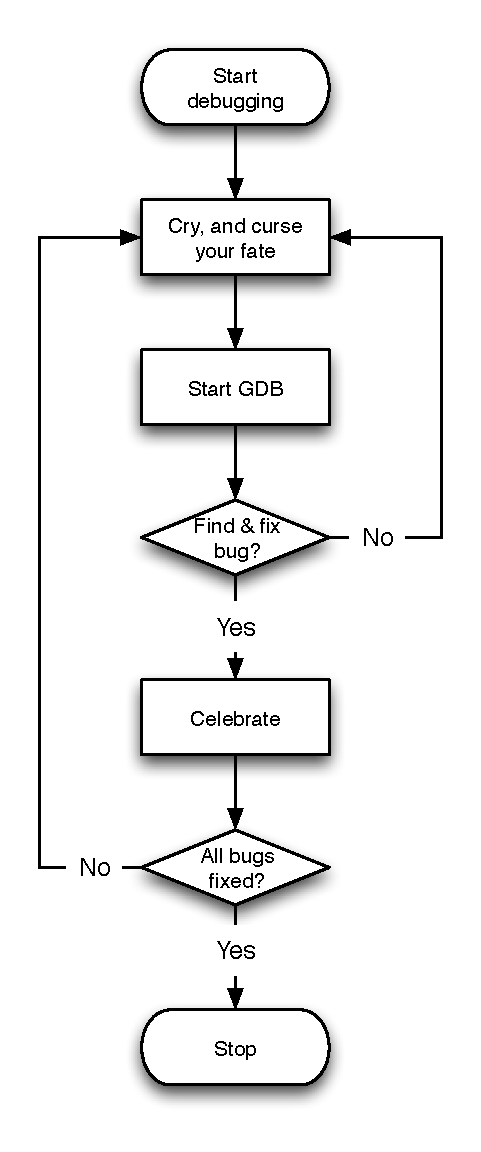
\includegraphics{FlowChart}}
    \caption{Figure caption}
    \label{FlowChart1}
\end{figure}
\end{verbatim}

\noindent
Which yields the figure in Fig.~\ref{FlowChart1}.  Note that the \verb+figure+
environment is one that I'm not going to explain; the only thing you
really need to know is that it forces whatever is inside of it to appear on
one page, which is exactly what you want with a picture.  If you're interested,
search on the web for it, otherwise, just copy the \LaTeX\ above, and replace
what you need.

\begin{figure}[htb]
    \centering
    \resizebox{1in}{!}{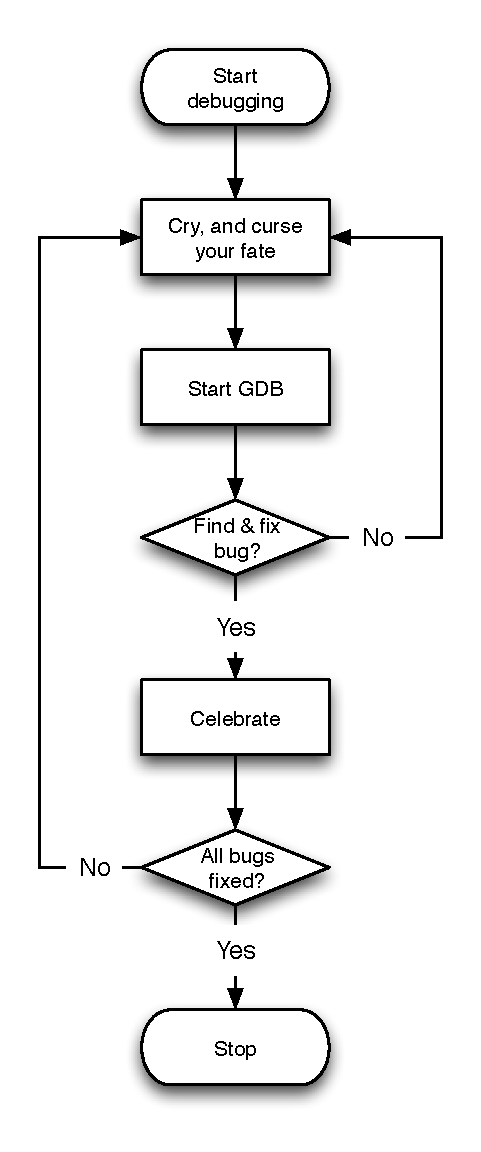
\includegraphics{FlowChart}}
    \caption{Debugging reality}
    \label{FlowChart1}
\end{figure}

\pagebreak
You can group multiple pictures together using the \verb+\subfloat{}+ 
command as in Fig~\ref{FlowChart2}.

\begin{verbatim}
\begin{figure}[htb]
    \centering
    \subfloat[Left debugging]
    {
        \resizebox{1in}{!}{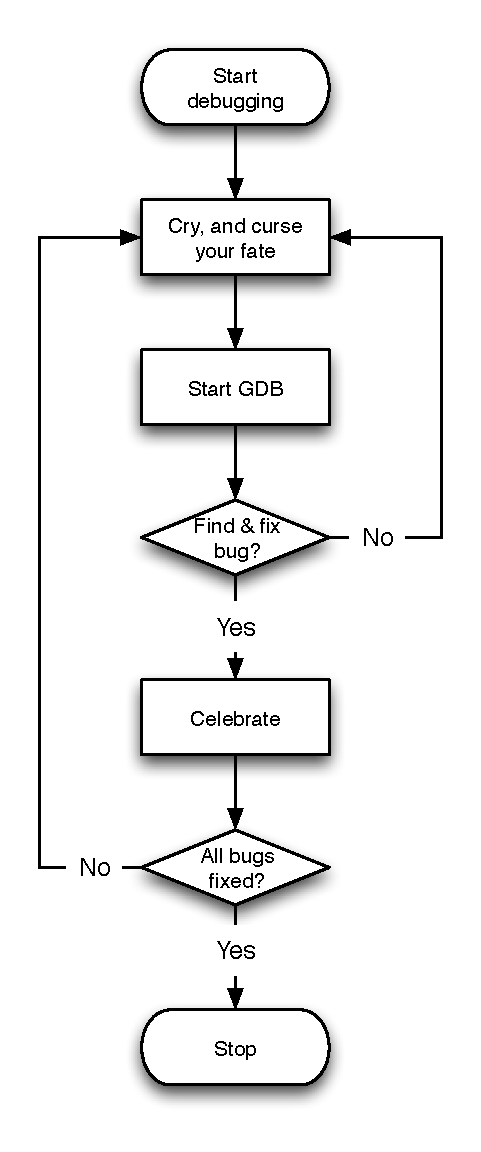
\includegraphics{FlowChart}}
        \label{FlowChart2a}
    }
    \subfloat[Right debugging]
    {
        \resizebox{1in}{!}{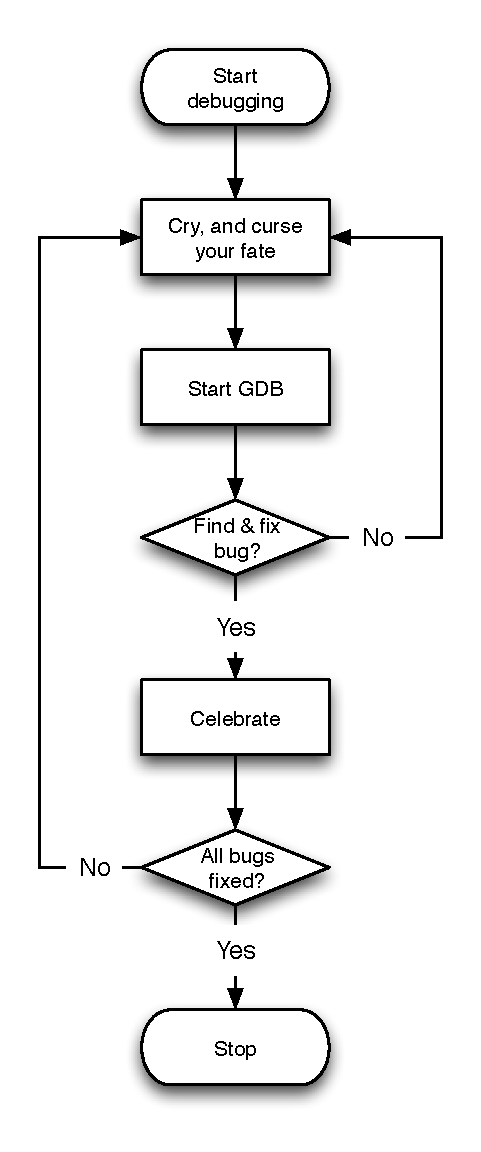
\includegraphics{FlowChart}}
        \label{FlowChart2b}
    }
\caption{Parallel debugging}
\label{FlowChart2}
\end{figure}
\end{verbatim}

\begin{figure}[htb]
    \centering
    \subfloat[Left debugging]
    {
        \resizebox{1in}{!}{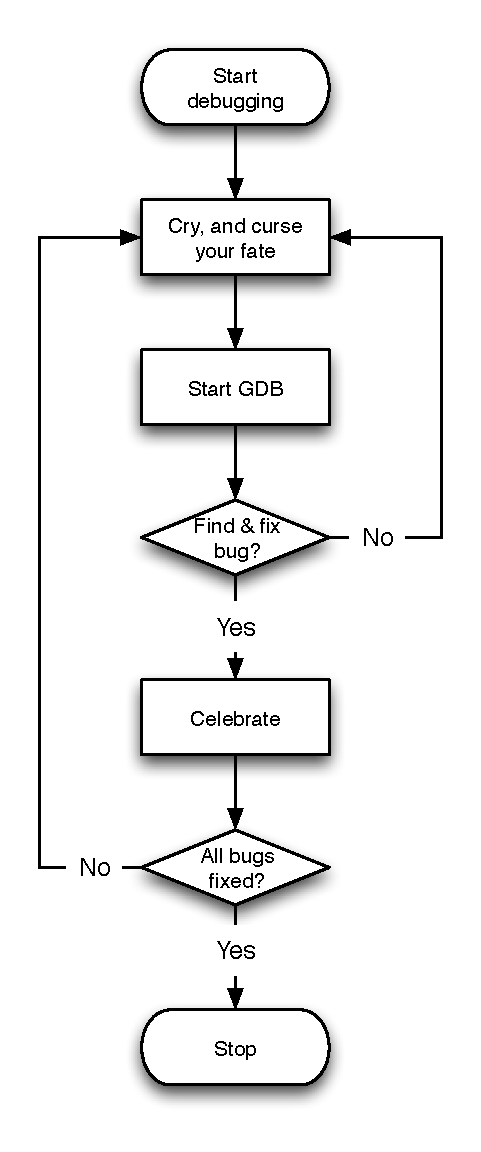
\includegraphics{FlowChart}}
        \label{FlowChart2a}
    }
    \subfloat[Right debugging]
    {
        \resizebox{1in}{!}{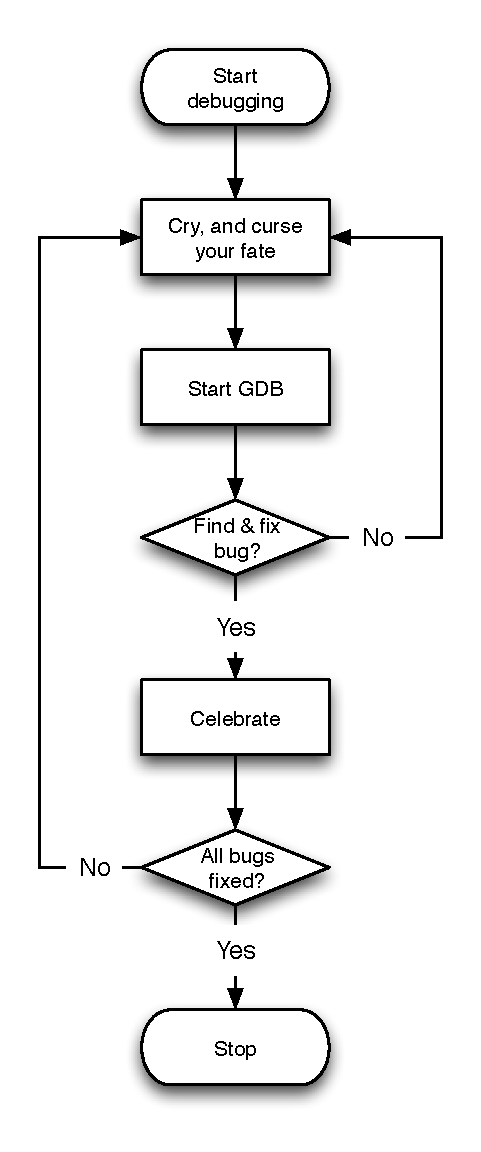
\includegraphics{FlowChart}}
        \label{FlowChart2b}
    }
\caption{Parallel debugging}
\label{FlowChart2}
\end{figure}

The line \verb+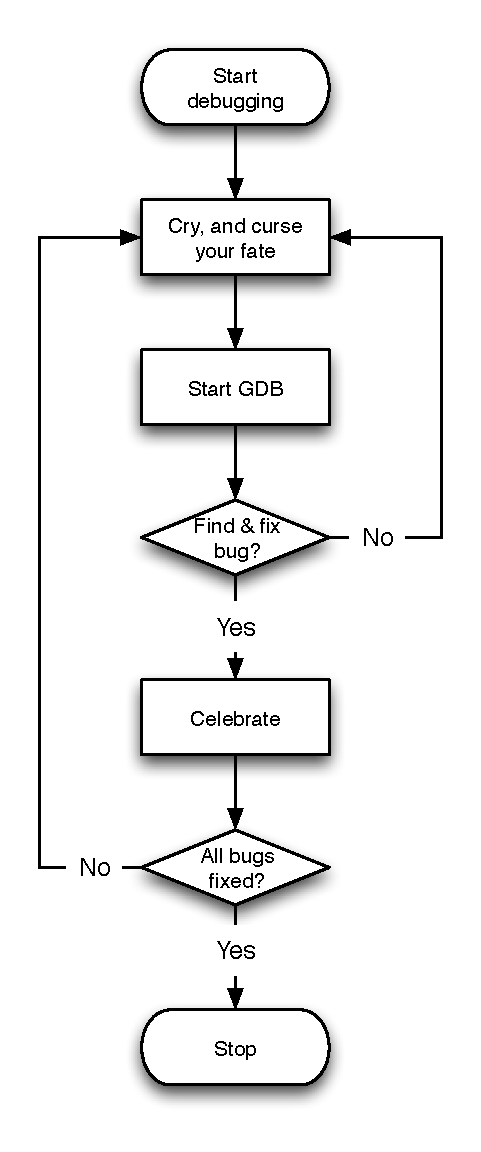
\includegraphics{FlowChart}+ tells \LaTeX\ to look for 
the file named \verb+FlowChart+ in the same directory as where your 
\LaTeX\ file is.  Note that there isn't a file suffix because at the top 
of the \\ \verb+LaTeX_Tutorial.tex+ file, I've included the command 
\verb+\DeclareGraphicsExtensions{.eps}+ (or possibly 
\verb+\DeclareGraphicsExtensions{.pdf}+, if I've forgotten to comment 
out the other line).  That command tells \LaTeX\ what the file suffix to 
search for is.

The \verb+\resizebox{1in}{!}{...}+ part tells \LaTeX\ that I want the 
image to be resized.  \verb+\resizebox+ uses 3 arguments; the first is 
the width you want, the second is the height you want, and the third is 
the thing you want resized (which can be objects other than graphics, 
but it is unlikely you'll use it for anything else).  The \verb+!+ in either 
of the first two arguments means that you want to keep the aspect ratio 
the same, so your graphic will shrink in size, but it won't get 
distorted.

The \verb+\label+ is described in Section~\ref{Cross References}.  As a 
general rule of thumb, every \verb+figure+ and every \verb+subfloat+ 
should have their own label.

Other arguments are caption text, and getting the figure centered 
correctly; play with the code to see what is going on.

\section{Cross References}
\label{Cross References}

To make a reference within a document, you use the \verb+\label{}+ and 
\verb+\ref{}+ commands.  The \verb+\label{}+ command acts like the 
anchor for a link, while the \verb+\ref{}+ command tells \LaTeX\ to make 
a link to a particular anchor.  Note that \verb+\label{}+'s are not 
exactly like URLs; they will only anchor to the start of a section.  If 
you go through the \texttt{LaTeX\_Tutorial.tex} file, you will see many 
uses of both of the commands.  Try moving them around a bit, and you'll 
see where you can put them.  You can put any non-special character in 
for labels, including spaces.  The labels can be as long as you wish, so try 
to make your labels descriptive, it will make it easier to find errors.

\section{Miscellaneous}
\label{Miscellaneous}

The \verb+\noindent+ command right before a paragraph will force the 
start of the line to be all the way to the left of the page.  Look in the
\texttt{LaTeX\_Tutorial.tex} file for examples of how its used.

\subsection{Whitespace}
\label{Whitespace}

There are a number of ways of adding more space to a line, and there are 
some ways of forcing \LaTeX\ to go backwards.  Here are a few space 
characters: 
\bigskip

\begin{tabular}{|c|c|} \hline 
\verb+\,+       & `\,'  \\ \hline
\verb+\;+       & `\;'  \\ \hline
`\verb+\ +'     & `\ '  \\ \hline
\verb+~+        & `~'   \\ \hline
\end{tabular}

\bigskip
\noindent
\verb+~+ is a non-breaking space character.  That means that if you have
two words next to each other, but separated by \verb+~+, they will be
treated as one word for the purposes of line breaking, justification, etc.
The practical upshot of this is if you have something like a reference
like \verb+Fig.~\ref{some reference}+, you are guaranteed that the
\verb+Fig.+ part and the generated reference number are always stuck
together.  This is handy if there is a line break, or a page break as you
are guaranteed that you don't end up with the \verb+Fig.+ on a different
line or page than the reference number.

\subsection{Vertical Spacing}

You can create a page break via the \verb+\pagebreak+ command.  Put it 
on any line by itself, and the page will be broken there.

You can make a line break via the \verb+\linebreak+ or \verb+\\+ 
commands, and \LaTeX\ will try to justify the lines.  \verb+\newline+ simply 
breaks the line, without trying to justify it.

\verb+\bigskip+, \verb+\medskip+, and \verb+\smallskip+ will put space 
between paragraphs.  This can be handy if you want to space a paragraph 
away from an equation, or some other object.

\section{Errors}

\LaTeX\ is powerful, but its error messages can range from useful to 
malignantly misleading.  You will get used to error messages on lines 
that can't possibly have errors on them, only to find that the error 
occurred somewhere far, far away.  The best thing to do is to run 
\LaTeX\ \emph{often}, and to keep everything under version control.  
That way, when something breaks, you can do a quick diff between your 
old and new versions, which should give you an idea as to where the 
errors could be.

Here are some common problems:

\begin{itemize}

\item \textbf{Incorrect or missing reference numbers} Try re-running 
\LaTeX.  \LaTeX\ uses a two pass algorithm to fill in all the reference 
details.  In the first pass, it builds a database of where the 
\verb+\labels{}+ are, and in the second pass, it actually puts those 
references into the \verb+\ref{}+s.  If that fails, \emph{make 
absolutely sure} that your references and labels match \emph{exactly}.  
That usually solves most problems.

\item \textbf{Complaints about a missing \$} You tried to use something 
that only has meaning inside of the math mode outside of it.  The most 
common cause of this is the `\_' character.  If you forget to escape it 
with a \verb+\+, then it will cause you a headache.  Note that the 
warning is generally on the wrong line, sometimes in the wrong part of 
your paper all together.  The easiest way to fix this is to use your 
favorite search utility to look for any unescaped `\_' characters, and 
then to try again.

This can also happen if you accidentally put a \verb+$+ inside of another 
math mode like so:

\begin{verbatim}
    \begin{equation}
    $E = mc^{2}$
    \end{equation}
\end{verbatim}

Double check all your math environments to see if you've forgotten anything,
or gotten overzealous and added extra environment markers.

\item \textbf{ANY complaint that occurs beyond the end of the document} 
Check to make sure that every open brace or bracket is matched with a 
close brace or bracket. Also make sure that every \verb+\left+ is 
matched with a \verb+\right+ and that every \verb+\begin{}+ is matched 
with an \verb+\end{}+.  Inevitably, there is something left open that 
needs to be properly closed off. Also make sure that everything is 
properly nested; incorrect nesting will cause you headaches as well. 
Finding it will likely be a hassle because \LaTeX\ won't tell you where 
your error actually occurred, so it will involved some detective work.  
Good luck, you're going to need it!

\item \textbf{I fixed the bug, \emph{why doesn't it work?!?!?}} Throw 
away all of the intermediate files that \LaTeX\ generated.  Those 
intermediate files are \LaTeX's cached state, and if a prior error has 
mangled that state somehow, \LaTeX\ usually won't be able to recover 
from it.  By throwing away those files, you'll force \LaTeX\ to rebuild 
from a clean state.

\end{itemize}

\end{document}
